\documentclass[runningheads,a4paper,fleqn]{llncs}

\usepackage{url}
\usepackage{amsmath}
\usepackage{amssymb}
\usepackage{alltt}
\usepackage{lineno}
\usepackage{graphicx}
\usepackage{subfigure}
\usepackage[normalem]{ulem}

\usepackage{tikz}
\usetikzlibrary{arrows,petri,topaths}
\usepackage{tkz-berge}

\begin{document}

\title{FlowArrays: Barrier-Free ParArrays}
\author{Tobias Schlatter\inst{1} \and Aleksandar Prokopec\inst{2} \and
  Heather Miller\inst{2} \and Philipp Haller\inst{2} \and Martin
  Odersky\inst{2}}

\authorrunning{Tobias Schlatter}

\institute{Student, EPFL \and Advisors, EPFL}

\graphicspath{{figs/}}

\maketitle

\begin{abstract}
  In \cite{FP12} we proposed an unordered, barrier- and lock-free,
  parallel datastructure, the FlowPools. The following attempts to
  implement a bigger application using FlowPools, showed that the lack
  of ordering is very limiting. The proposed FlowArrays do not have
  this limitation: Having a very similar structure than ParArrays
  \cite{collect11}, FlowArrays eliminate the need to block inbetween
  monadic operations on ParArrays while exposing a very similar
  interface to the programmer.
  %% TODO write about performance
\end{abstract}

\section{Introduction}
%% This is the usual blah about nothing but which is required...


\section{Overview}
In this section we'll first outline how FlowArrays try to improve on
ParArrays from an abstract perspective. Then we'll show some of the
difficulties that arise particularly with this aproach. The next
section (c.f. page~\pageref{sec:implementation}) will explain in more
detail, how FlowArrays are implemented.

The evaluation section (c.f. page~\pageref{sec:evaluation}) will
analyze the performance of FlowArrays.
%% TODO write more

\subsection{Barrier-Freedom}
FlowArrays in comparison to ParArrays are barrier-free: We'll
illustrate on the simplest example, a single \texttt{map} map
operation, how these two datastructures differ.

Let's consider the following code for ParArrays and
FlowArrays. Fig.~\ref{fig:barrier-free} shows a schematic
illustration of what's going on.

\noindent
\begin{minipage}[t]{.5\textwidth}
\begin{alltt}
{\scriptsize
val pa1 = ParArray.tabulate(n)(x => x*x)
val pa2 = pa1.map(_ * 2)
}
\end{alltt}
\end{minipage}
\begin{minipage}[t]{.5\textwidth}
\begin{alltt}
{\scriptsize
val fa1 = FlowArray.tabulate(n)(x => x*x)
val fa2 = fa1.map(_ * 2)
}
\end{alltt}
\end{minipage}

In both cases, we first create a Par/FlowArray using a tabulate. Both
Par- and FlowArrays will use exponential task splitting
\cite{collect11,cong08} to distribute the workload of calculating the
individual elements. The crucial difference between ParArrays and
FlowArrays starts here: With ParArrays, the call to \texttt{tabulate}
(and any other function for that matter) will only return, once every
element has been calculated. In contrast, the call to
\texttt{tabulate} on FlowArrays will return immediately, yielding an
array whose elements are specified, but not yet calculated.

When calling \texttt{map} on the first Par/FlowArray, this difference
becomes even clearer: ParArrays will do the same thing as for
\texttt{tabulate}: Split up the task of calculation and start right
away. FlowArrays however, will align the task blocks and start
calculating the elements, once the elements the result depends on have
been calculated (in our case the result of the \texttt{tabulate}). So
contrary to ParArrays, FlowArrays are able to start subsequent
calculations partially, even if not all the elements of the original
array have been calculated.

\begin{figure}
  \centering
  \subfigure[ParArray] {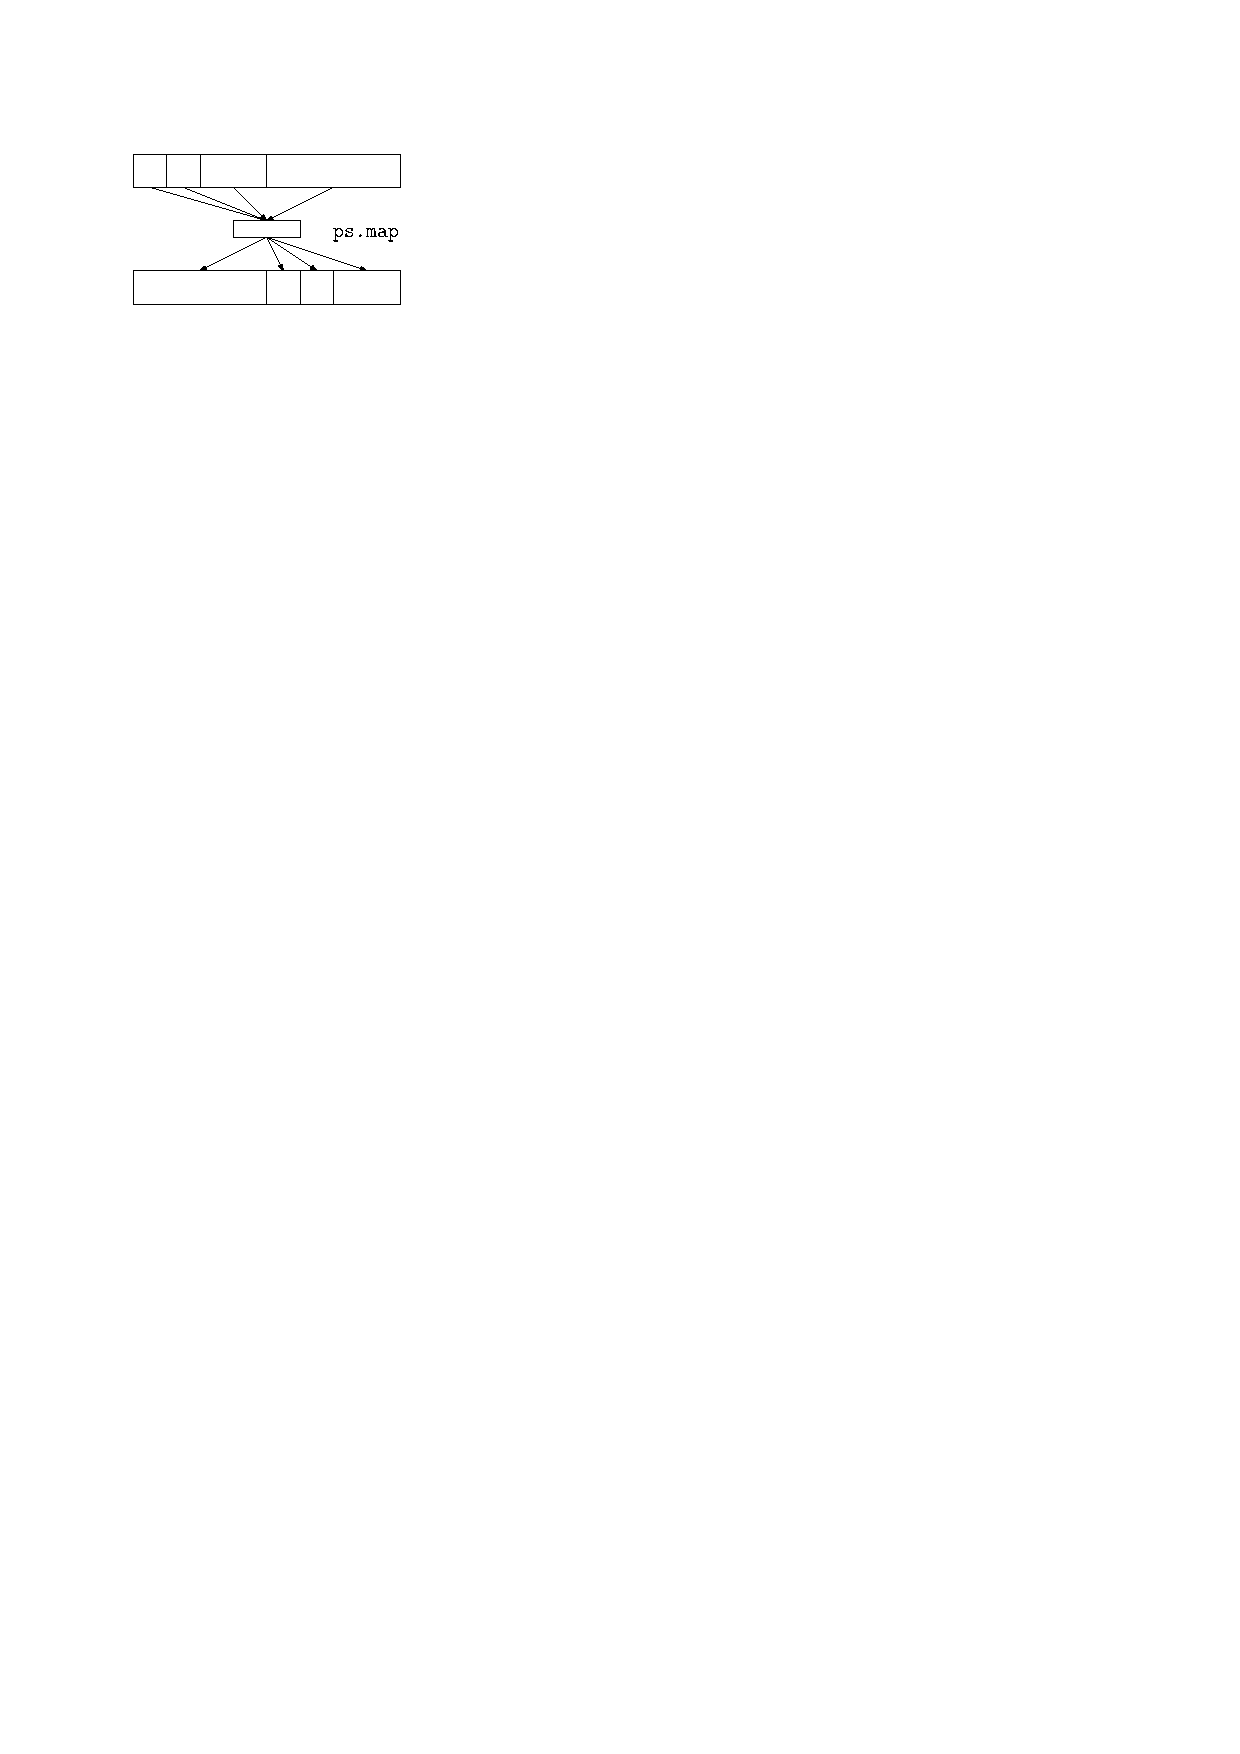
\includegraphics{barrier-free-pa}}
  \qquad
  \subfigure[FlowArray]{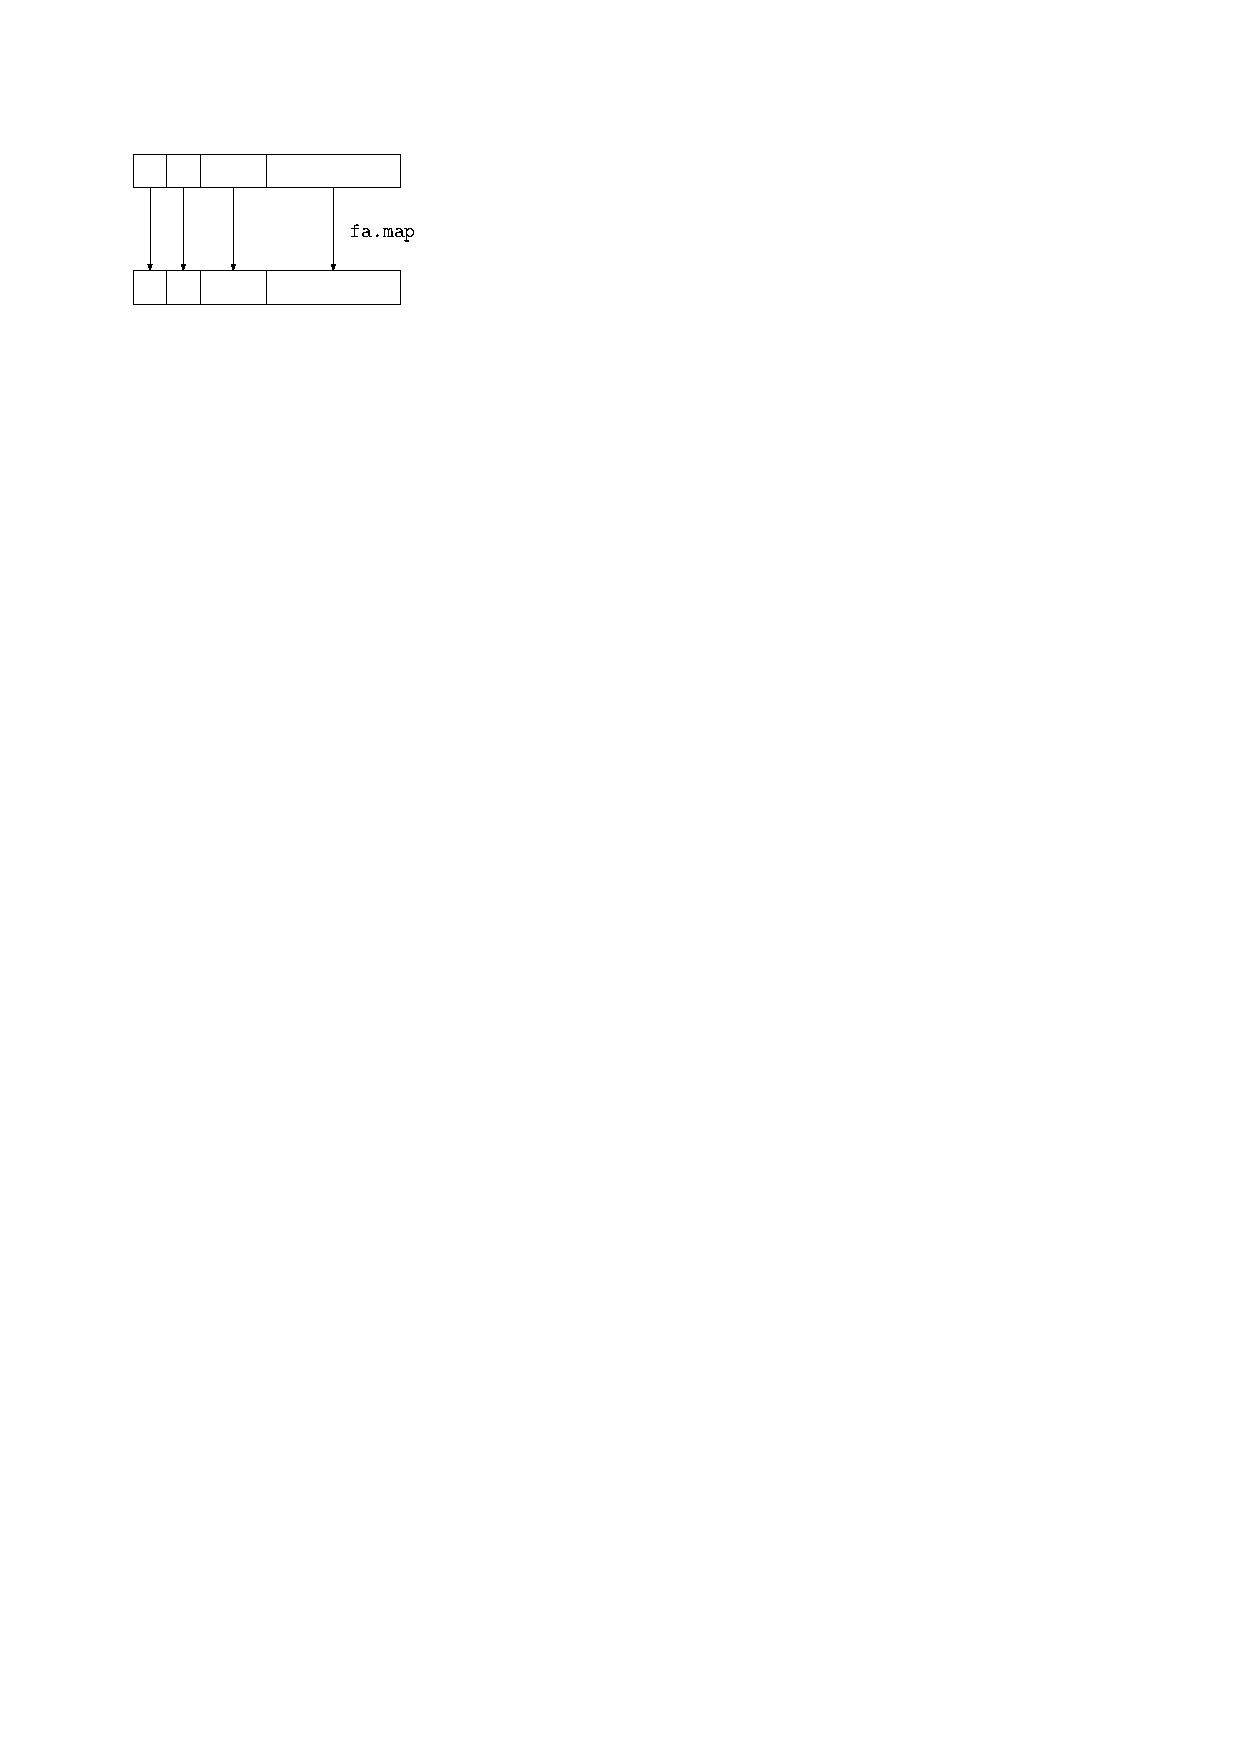
\includegraphics{barrier-free-fa}}
  \caption{Illustration of barrier-freedom of FlowArrays}
  \label{fig:barrier-free}
\end{figure}

\subsection{Dependency Tracking}
We'll now describe in detail what happens, when a \texttt{map} is
called on a FlowArray depending on the different possible states of
its blocks. Fig~\ref{fig:dep-track} illustrates the different
scenarios that may happen. In the figure, the circles represent jobs:
grey if executing or submitted to the execution queue, white if
waiting in an internal queue of another job (indicated by the dashed
arrow). The rectangles represent data blocks of a FlowArray: white if
(partially) empty, grey if fully calcuated.

When a \texttt{map} is called on a FlowArray, each block chain will
start in one of the three first states and then propagate to the right
until both blocks are fully calculated. The cases are the following:

\begin{figure}
  \centering
  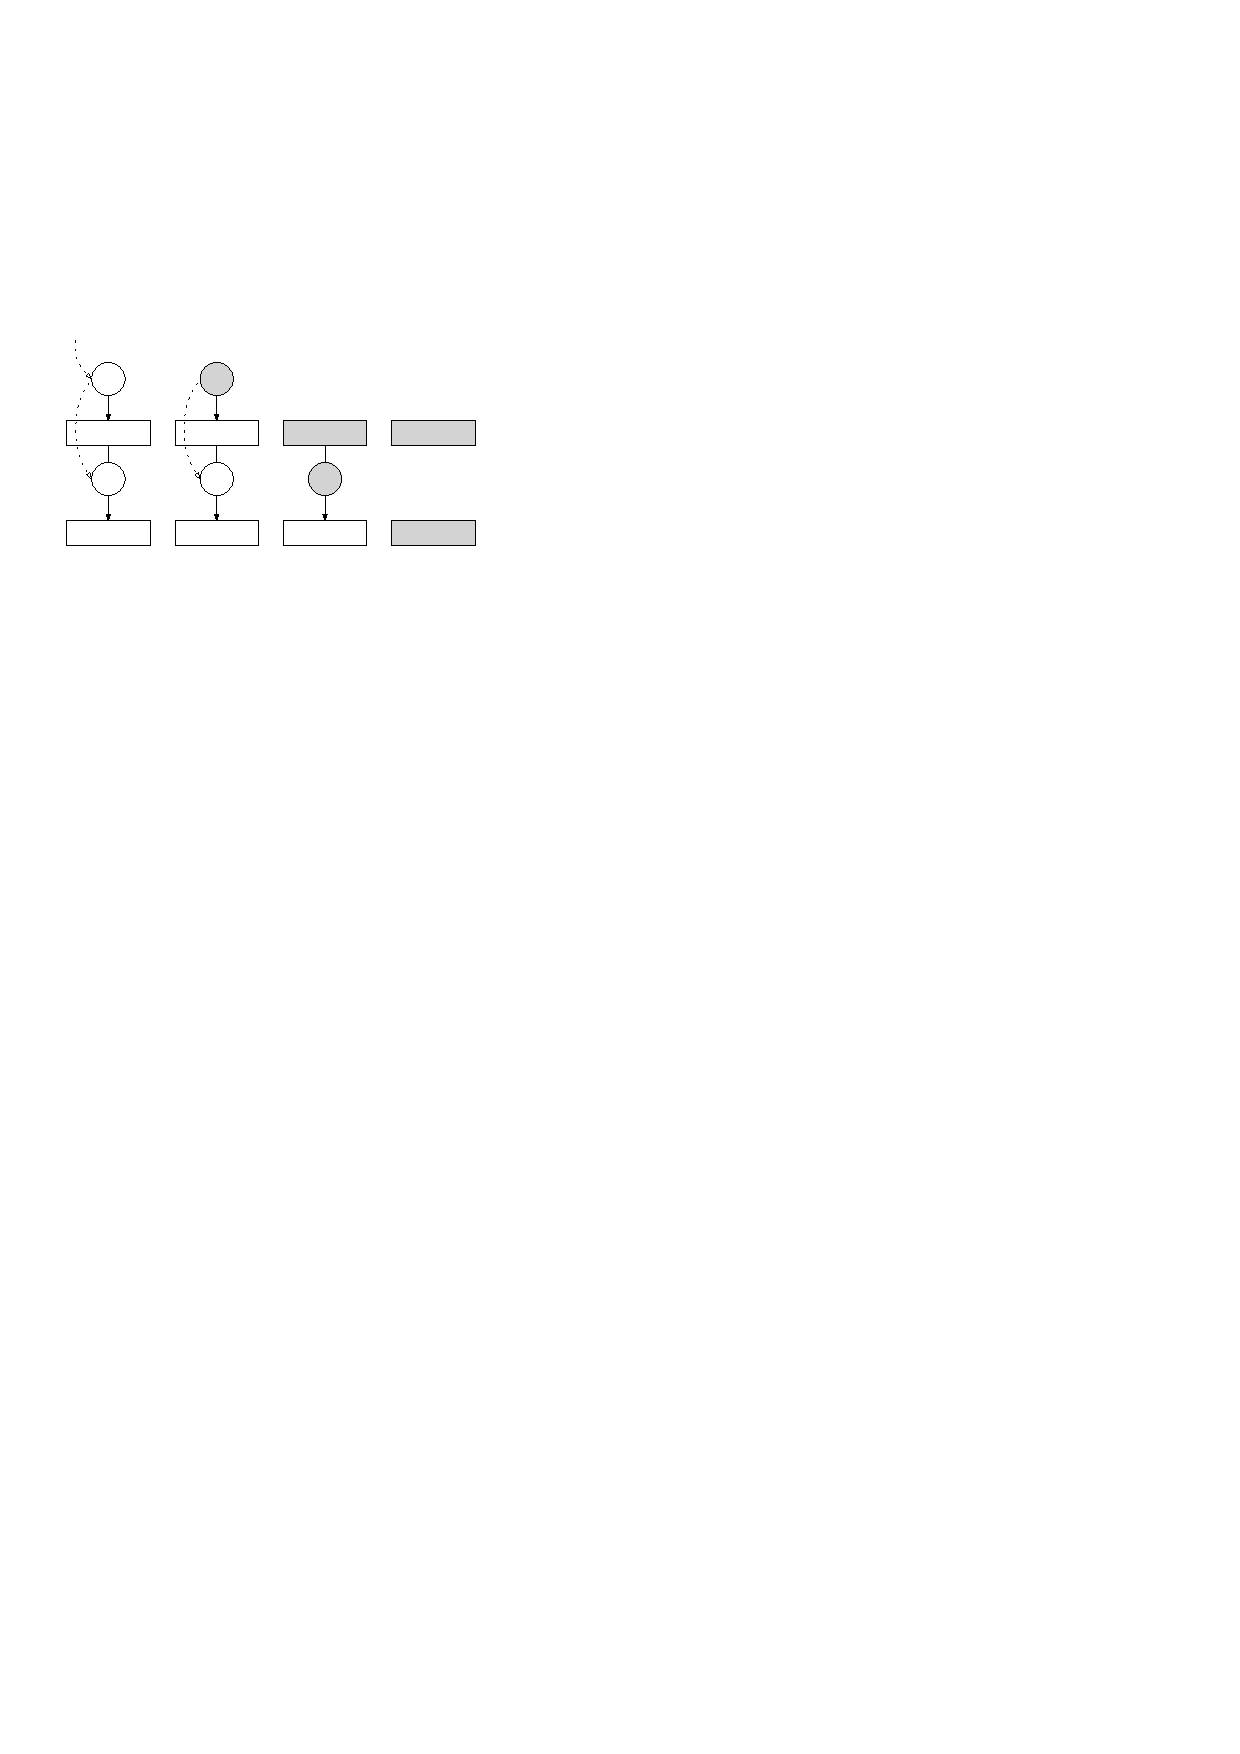
\includegraphics{dependency-tracking}
  \caption{Illustration of the dependency tracking in FlowArrays}
  \label{fig:dep-track}
\end{figure}


\begin{enumerate}
\item Both blocks are not yet calculated and the job for the first
  block still depends on some other job: The second job is added to
  the first job's dependency queue.
\item The job for the first block is scheduled for execution but not
  yet finished: The second job is added to the first job's dependency
  queue.
\item Calculation of the first block is already completed: The second
  job is scheduled for execution immediately.
\item Both blocks are completely calculated.
\end{enumerate}

\subsection{Operations}
We have seen how dataflow with dependency tracking can be used in
monadic operations on the example of a \texttt{map}. In this section
we'll describe the caveats of other common monadic operations on
arrays.

\subsubsection{Fold}
When doing out of order folding, each block has first to be reduced to
a single element, then these results have to be combined to the final
result. During splitting of the jobs, one can create a binary tree of
blocks along which one can later accumulate the elements;
fig~\ref{fig:fa-fold} illustrates this approach.

\begin{figure}
  \centering
  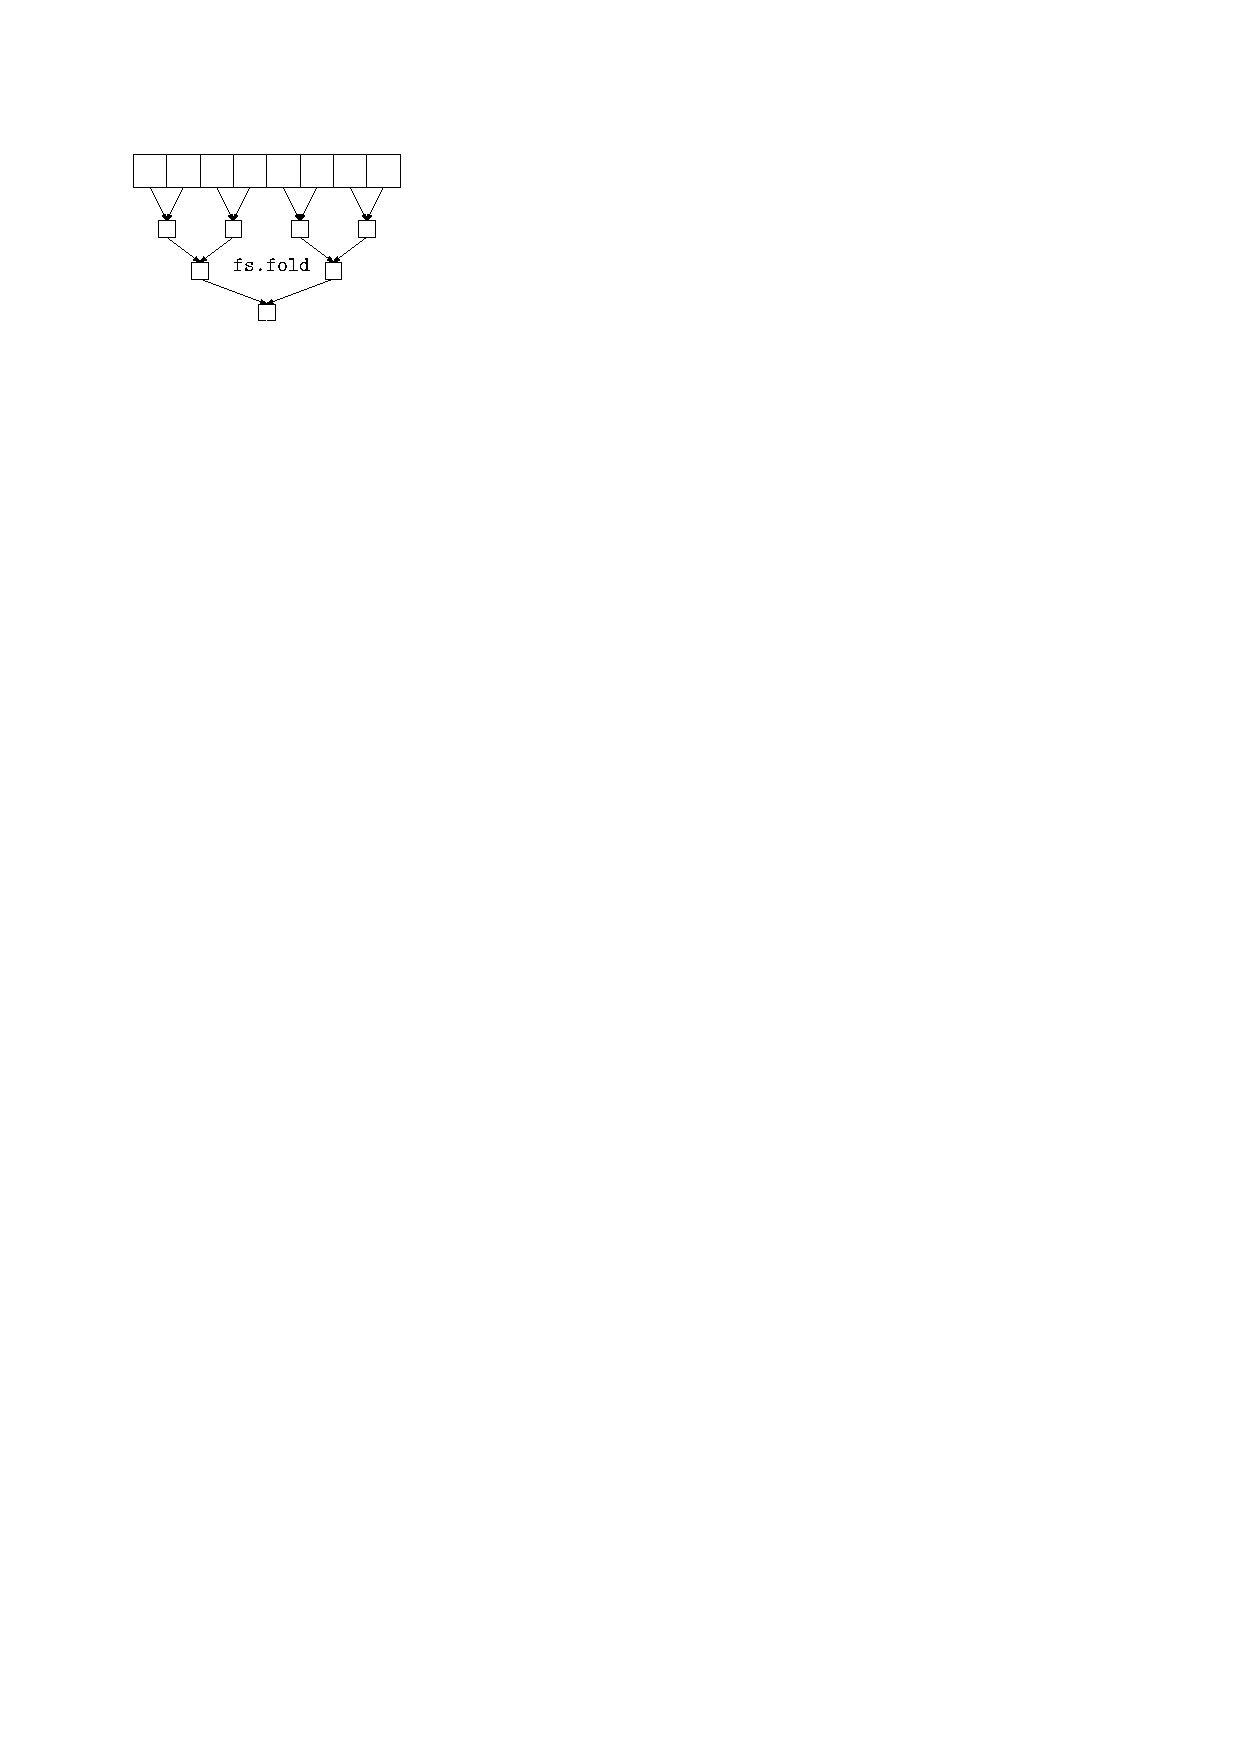
\includegraphics{fa-fold}
  \caption{Illustration of \texttt{fold} on a FlowArray}
  \label{fig:fa-fold}
\end{figure}

In order to keep the number of jobs (and hence the burden of managing
them) minimal, rather then spawning a single job for each accumulation
step in the tree, the job which finishes second on each node is
responsible to calculate its accumulated value. Using this scheme, the
same number of jobs are spawned as for a \texttt{map}.

Note that this approach is preferable to a single element where
completed elements aren accumulated using a CAS since the former
does preserve the order in which elements are accumulated. I.e. it
requires the accumulation function to be associative, not
commutative.

\subsubsection{FlatMap}

When calling flatMap on a FlowArray, the size of the resulting
FlowArray is not known until the inner FlowArrays are created and
hence their size can be read. However, since this happens
asynchronously, the size of the resulting FlowArray would not be known
at its creation. This poses several challenges:

\begin{itemize}
\item The interface of FlowArrays becomes more complex
\item Increased difficulty in memory allocation
\item Increased difficulty in scheduling of subsequent calls
\end{itemize}

Instead of deferring the size calculation, FlowArrays require to pass
the size of the resulting FlowArrays of a \texttt{flatMap} operation
when calling it. This greatly facilitates further handling --
especially scheduling -- of the resulting FlowArray.

Further, the FlowArray now needs to keep track of dependencies twice:
Once, whether a sub-FlowArray has already been created, second,
whether a given one of its blocks is already calculated. Refer to
fig~\ref{fig:flatMap-dependency} for an illustration. This tracking
requires the outer FlowArray to keep references to all the created
ones. In order to avoid unnecessary copying of data, the FlowArray
remains in this hierarchical structure instead of being truly
flattened.

\begin{figure}
  \centering
  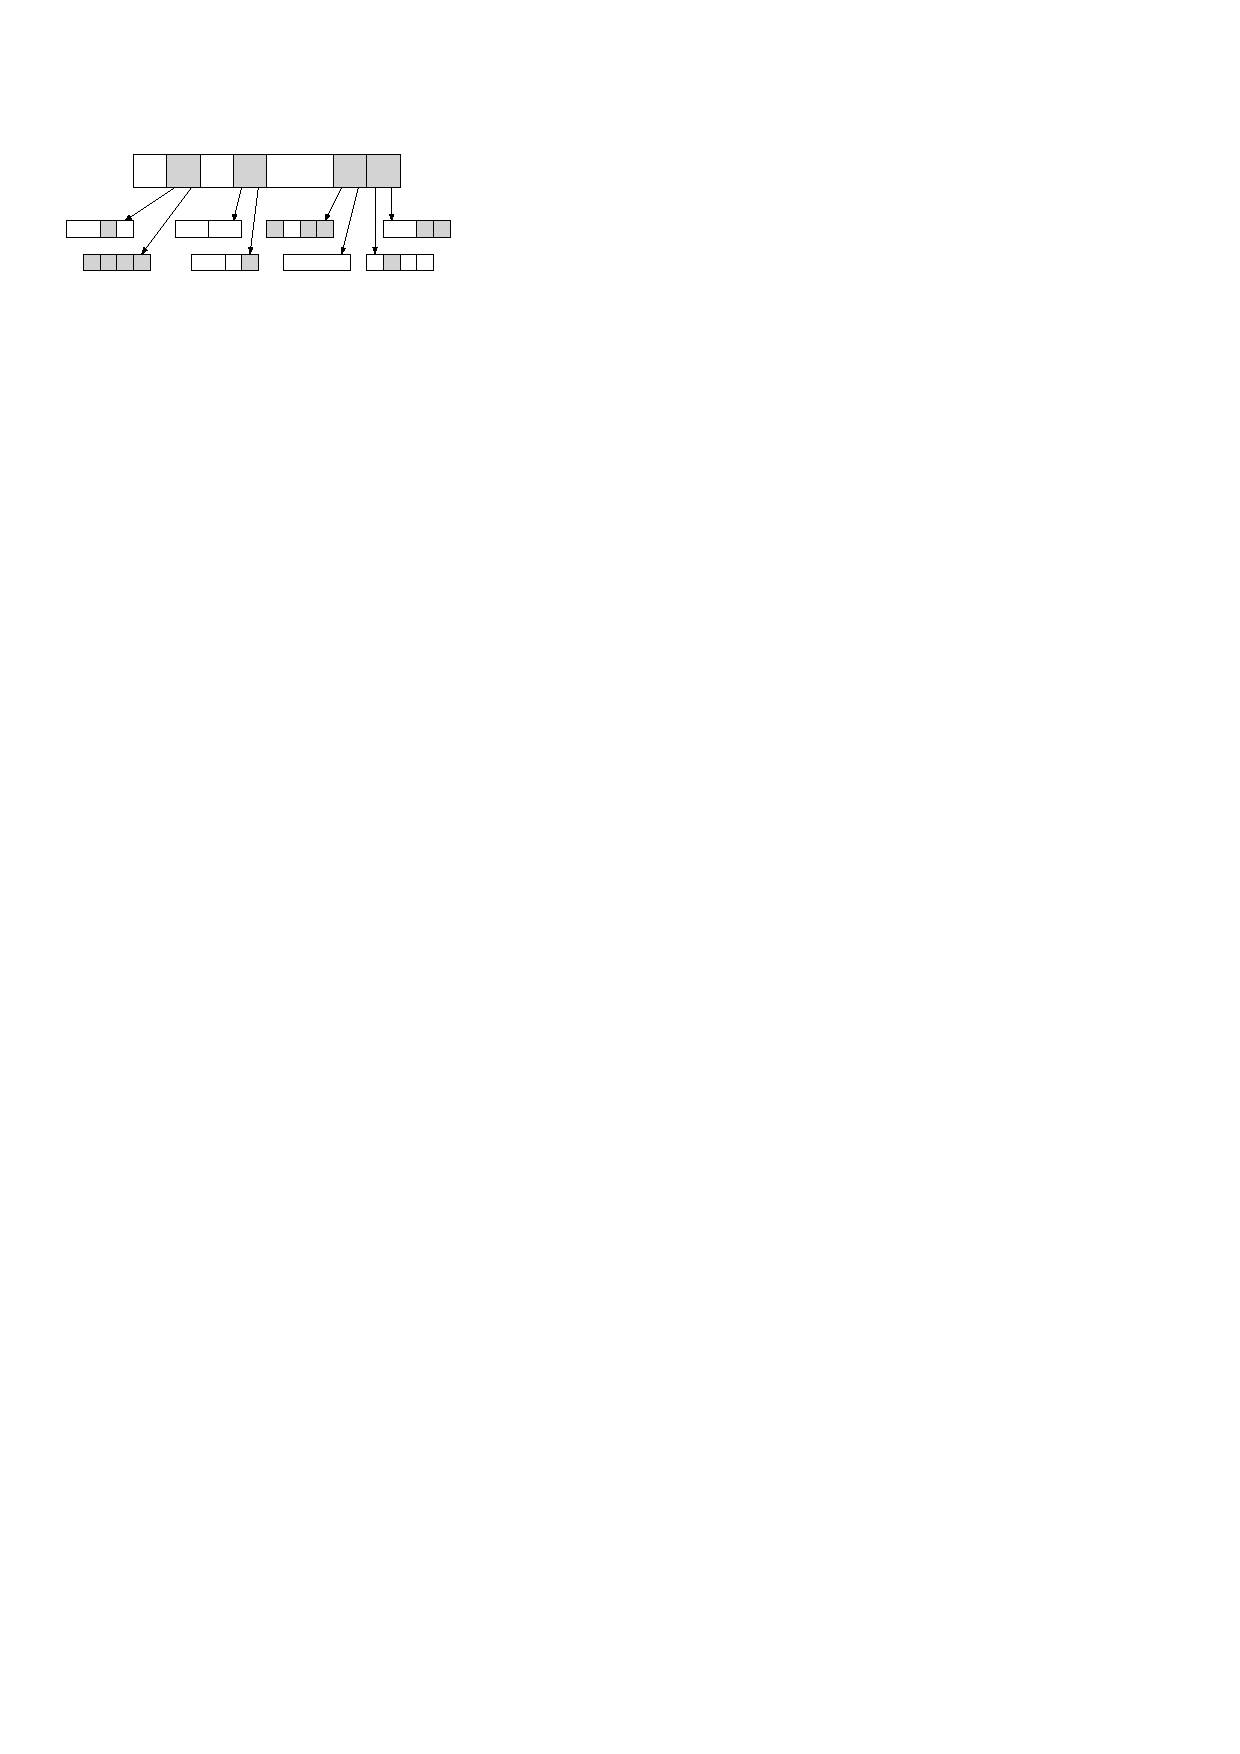
\includegraphics{flatMap-dependency}
  \caption{Illustration of depenceny-tracking requirements in a
    Hierarchical FlowArray resulting from a \texttt{flatMap}}
  \label{fig:flatMap-dependency}
\end{figure}

When a \texttt{map} is called on one of these \emph{Hierarchical
  FlowArrays} individual \texttt{maps} are called for each sub array
and only then the resulting data is written in a flat array. This
allows to ``flatten out'' those hierarchical structures without
additional computation costs. Note that this scheme does require the
blocks to be re-aligned at a later point in time to remove the
arbitrary splitting imposed by the hierarchy introduced by the
\texttt{flatMap}. For details how block splitting is propagated
through dependencies, please refer to
section~\ref{sec:implementation}.

\subsubsection{Zip}
When zipping, again we impose a restriction on the size: the size of
the two FlowArrays which are being zipped need to be of the same
size. This is again to ease scheduling and implementation. However, in
this case, minor changes in the implementation could easily remove
this limitation (unlike \texttt{flatMap}, where the interface would
need to undergo a fundamental change).

Further, the splitting of the two FlowArrays which are being zipped
may be totally different, e.g. due to a preceding \texttt{flatMap} on
one of them. Hence -- again -- re-alignment of blocks is required,
before the zipped tuples can be created.

\section{Implementation}
\label{sec:implementation}

\subsection{FlowArray Jobs}

\subsection{Slice Views}

\subsection{Hierarchical FlowArrays}

\section{Evaluation}
\label{sec:evaluation}

\section{Conclusion}

\bibliographystyle{abbrv}
\bibliography{bib}

\end{document}

%%% Local Variables: 
%%% mode: latex
%%% TeX-master: t
%%% End: 
